\documentclass[10pt,twocolumn]{exam}
\usepackage[hon]{template-for-exam}
\usepackage{endnotes,graphicx}
\usepackage{tikz,tikzpingus,graphicx}
%\pinguloadlibrary{horse}
\usetikzlibrary{shadings,decorations.pathmorphing,arrows.meta,patterns}
\def\answer#1{\footnotetext{#1}}
\def\theanswers{\theendnotes}
\def\myquestion{\question\stepcounter{footnote}}
%\def\enoteheading{Answer}

\title{Chapters 4 and 5 Homework}
\author{Rohrbach}
\date{\today}

\begin{document}
\maketitle

\noindent
\textit{Questions and figures are from OpenStax} College Physics \textit{2nd ed, unless otherwise noted.}

\vspace{-1em}

\begin{questions}

\uplevel{\section*{Forces \& Newton's Laws}}

  \myquestion 
    (OpenStax Ex 4.1) A 63.0-kg sprinter starts a race with an acceleration of 4.20 m/s$^2$. What is the net external force on him? \answer{265 N}

  % \myquestion 
  %   (OpenStax Ex 4.2) If the sprinter from the previous problem accelerates at that rate for 20 m, and then maintains that velocity for the remainder of the 100-m dash, what will be his time for the race? \answer{9.26 s (a record!)}

  \myquestion
    (OpenStax Ex 4.10) A powerful motorcycle can produce an acceleration of 3.50 m/s$^2$ while traveling at 90.0 km/h. At that speed the forces resisting motion, including friction and air resistance, total 400 N. (Air resistance is analogous to air friction. It always opposes the motion of an object.) What is the magnitude of the force the motorcycle exerts backward on the ground to produce its acceleration if the mass of the motorcycle with rider is 245 kg? \answer{1260 N} 

  \myquestion
    \textbf{Bonus!} (OpenStax Ex 4.44) When starting a foot race, a 70.0-kg sprinter exerts an average force of 650 N backward on the ground for 0.800 s. (a) What is his final speed? (b) How far does he travel?

  \begin{enumerate}
    \item[CQ2)] What properties do forces have that allow us to classify them as vectors?
    \item[CQ3)] How are inertia and mass related?
    \item[CQ4)] What is the relationship between weight and mass? Which is an intrinsic, unchanging property of a body?
    \item[CQ5)] Which statement is correct? (a) Net force causes motion. (b) Net force causes change in motion. Explain your answer and give an example.
    \item[CQ6)] Why can we neglect forces such as those holding a body together when we apply Newton's second law of motion?
    \item[CQ8)] Describe a situation in which the net external force on a system is not zero, yet its speed remains constant.
    
    \pagebreak
    \vspace*{2.9em}

    \item[CQ10)] A rock is thrown straight up. What is the net external force acting on the rock when it is at the top of its trajectory?
    \item[CQ15)] When you take off in a jet aircraft, there is a sensation of being pushed back into the seat. Explain why you move backward in the seat—is there really a force backward on you? (The same reasoning explains whiplash injuries, in which the head is apparently thrown backward.)
    \item[CQ18)] Why does an ordinary rifle recoil (kick backward) when fired? The barrel of a recoilless rifle is open at both ends. Describe how Newton's third law applies when one is fired. Can you safely stand close behind one when it is fired?
    \item[CQ-A)] (Original Question) A horse pulls a cart with a force of 400 Newtons forward.  However, according to Newton's Third Law, whenever the horse pulls the cart, there is an equal and opposite reaction of the cart pulling the horse.  Therefore, the cart pulls the horse with a force of 400 Newtons backward.  How does the cart move?  Shouldn't those two forces cancel each other out giving to a net force of zero?

    \tikzstyle{wheel}=[line width=10pt, fill=white]

    \begin{figure}[ht]
      \centering
      \renewcommand{\thefigure}{A}
      \begin{tikzpicture}[scale=0.3]
        \pingu[on horse,body=white, body front=white,small size, left eye color=white, right eye color=white,feet color=brown,bill color=white]
        \draw[rounded corners, fill=gray] 
          (0,-2) rectangle ++(7,-0.5);
        \draw[rounded corners, fill=gray] 
          (6,-1) -- ++(7,0) -- ++(-1,-4) -- ++(-5,0) -- cycle;
        \draw[wheel] (7,-5) circle (1);
        \draw[wheel] (12,-5) circle (1);
        \fill[pattern=north east lines] (-6,-6.3) rectangle ++(21, -0.5);
      \end{tikzpicture}
      \caption{Original Diagram. A horse and cart.}
    \end{figure}

    \item[CQ-B)] (Original Question) According to Newton's Third Law, when you jump off a desk, the force the Earth exerts on you, is equal to the force you exert on the Earth. However, it seems as if only you accelerate down. The earth doesn't seem to accelerate up. Why is this?
  \end{enumerate}

  \vs
  \pagebreak


\uplevel{\section*{Single-Body}}

  \myquestion 
    (OpenStax Ex 4.5) In Figure 4-7 below, the net external force on the 24-kg mower is stated to be 51 N. If the force of friction opposing the motion is 24 N, what force $F$ (in newtons) is the person exerting on the mower? Suppose the mower is moving at 1.5 m/s when the force $F$ is removed. How far will the mower go before stopping? \answer{75 N; 1.1 m}
    %
    \begin{figure}[h]
      \centering
      \renewcommand{\thefigure}{4.7}
      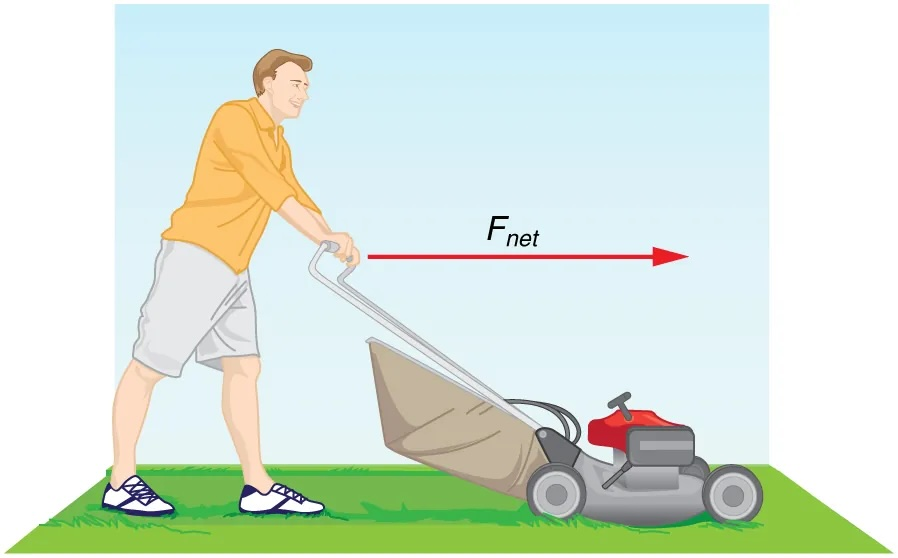
\includegraphics[width=2.1in]{OpenStaxImages/4-7.jpg}
      \caption{The net force on a lawn mower is 51 N to the right.}
    \end{figure}

  \myquestion 
    (OpenStax Ex 4.9) Suppose two children push horizontally, but in exactly opposite directions, on a third child in a wagon. The first child exerts a force of 75.0 N, the second a force of 90.0 N, friction is 12.0 N, and the mass of the third child plus wagon is 23.0 kg. \answer{(c) \SI{0.130}{m/s^2}; (d) \SI{0}{m/s^2}} (a) What is the system of interest if the acceleration of the child in the wagon is to be calculated? (b) Draw a free-body diagram, including all forces acting on the system. (c) Calculate the acceleration. (d) What would the acceleration be if friction were 15.0 N?
  
  \myquestion 
    (OpenStax Ex 4.13) The weight of an astronaut plus their space suit on the Moon is only 250 N. How much do they weigh on Earth? What is the mass on the Moon? On Earth? (The acceleration of gravity on the moon is 1.62 m/s$^2$) \answer{1500 N}

  \myquestion
    (OpenStax Ex 4.14) Suppose the mass of a fully loaded module in which astronauts take off from the Moon is 10,000 kg. The thrust of its engines is 30,000 N and the acceleration of gravity on the moon is 1.62 m/s$^2$. (a) Calculate its the magnitude of acceleration in a vertical takeoff from the Moon. (b) Could it lift off from Earth? If not, why not? If it could, calculate the magnitude of its acceleration. \answer{(a) \SI{1.38}{m/s^2}; (b) cannot take off}

  \myquestion
    \textbf{Bonus!} (OpenStax Ex 4.23) A $5.00\times10^5$-kg rocket is accelerating straight up. Its engines produce $1.250\times10^7$ N of thrust, and air resistance is $4.50\times10^6$ N. What is the rocket's acceleration? Explicitly show how you follow the steps in the Problem-Solving Strategy for Newton's laws of motion. 


  \begin{enumerate}
    \item[CQ23)] To simulate the apparent weightlessness of space orbit, astronauts are trained in the hold of a cargo aircraft that is accelerating downward at $g$. Why will they appear to be weightless, as measured by standing on a bathroom scale, in this accelerated frame of reference? Is there any difference between their apparent weightlessness in orbit and in the aircraft?
  \end{enumerate}

\vspace{-1em}
\uplevel{\section*{Multi-Body}}


  \myquestion
     (OpenStax Ex 4.22) Consider the baby being weighed in Figure 4.33. (a) What is the mass of the child and basket if a scale reading of 55 N is observed? (b) What is the tension $T_1$ in the cord attaching the baby to the scale? (c) What is the tension $T_2$ in the cord attaching the scale to the ceiling, if the scale has a mass of 0.500 kg? (d) Draw a sketch of the situation indicating the system of interest used to solve each part. The masses of the cords are negligible. \answer{(a) \SI{5.6}{kg}; (b) \SI{55}{N}; (c) 60 N}

      \begin{figure}[h]
        \centering
        \renewcommand{\thefigure}{4.33}
        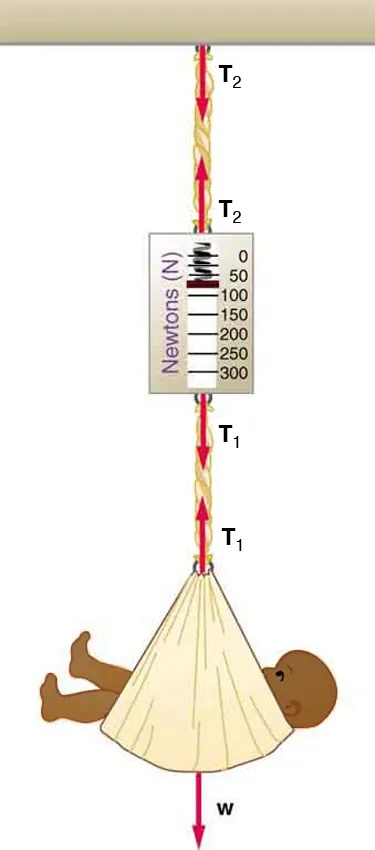
\includegraphics[height=2.2in]{OpenStaxImages/4-33.jpg}
        \caption{A baby is weighed using a spring scale.}
      \end{figure}


  \myquestion \label{hero1}
     (OpenStax Ex 4.34) Figure 4.38 shows Superhero and Trusty Sidekick hanging motionless from a rope. Superhero's mass is 90.0 kg, while Trusty Sidekick's is 55.0 kg, and the mass of the rope is negligible. (a) Draw a free-body diagram of the situation showing all forces acting on Superhero, Trusty Sidekick, and the rope. (b) Find the tension in the rope above Superhero. (c) Find the tension in the rope between Superhero and Trusty Sidekick. Indicate on your free-body diagram the system of interest used to solve each part. \answer{(b) \SI{1420}{N}; (c) 539 N}

    
  \myquestion \label{hero2}
    (Original question) The top rope in Figure 4.38 is attached to the bottom of an elevator that begins to accelerate upward.  The tension of the top rope increases to 1600~N. (a) Calculate the tension on the rope between Superhero and Trusty Sidekick. (b) Calculate the acceleration of the two heroes. \answer{(a) \SI{607}{N}; (b) \SI{1.23}{m/s^2}}

    \begin{figure}[h]
      \centering
      \renewcommand{\thefigure}{4.38}
      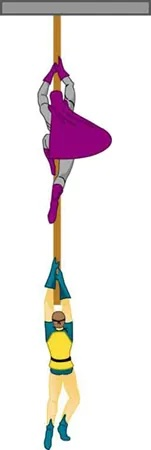
\includegraphics[width=0.9in]{OpenStaxImages/4-38.jpg}
      \caption{For problems~\ref{hero1}~\&~\ref{hero2}.  Superhero (at the top) is 90.0~kg; Trusty Sidekick (on the bottom) is 55.0~kg.  The ropes are massless.}
    \end{figure}

  \vs
  \pagebreak
  
  \myquestion \label{ModAtwood}
    (Original question) A block of mass $m_1=6.0$~kg rests on a frictionless horizontal table. The block is connected by a light, inextensible string that passes over a frictionless pulley to a hanging block of mass $m_2=4.0$ kg. \answer{(b) \SI{3.92}{m/s^2}; (c) \SI{23.52}{N}}
    %
    \begin{parts}
      \part Draw a free-body diagram for each block.
      \part Determine the acceleration of the system.
      \part Find the tension in the string.
    \end{parts}

    \tikzstyle{box}=[rounded corners,draw,minimum height=1cm]

    \begin{figure}[h]
      \centering
      \renewcommand{\thefigure}{B}
      \begin{tikzpicture}
        \node[box,minimum width=1.5cm] (one) at (0,0) {$m_1$};
        \node[box] (two) at (3.75,-3) {$m_2$};
        \draw[very thick] (one.east) -- (3.5,0) arc (90:0:0.25) -- (two);
        \fill[pattern=north east lines] (-3,-0.5) rectangle
          ++(6,-0.25);
        \draw (-3,-0.5) -- 
          ++(6,0) coordinate (edge) -- 
          ++(0,-1);
        \draw (edge) -- (3.5,-0.25) circle (0.25);
      \end{tikzpicture}
      \caption{Original Diagram. Figure for problem~\ref{ModAtwood}.}
    \end{figure}


  \myquestion \label{Atwood}
    (Original question) Two blocks of masses $m_1=5.0$~kg and $m_2=3.0$~kg are connected by a light, inextensible string that passes over a frictionless pulley. The system is released from rest. \answer{(b) \SI{2.45}{m/s^2}; (c) \SI{36.75}{N}}
    %
    \begin{parts}
      \part Draw a free-body diagram for each block.
      \part Determine the acceleration of the system.
      \part Find the tension in the string.
    \end{parts}

    \begin{figure}[h]
      \centering
      \renewcommand{\thefigure}{C}
          \begin{tikzpicture}
            \node[box] (one) at (-.75,0) {$m_1$};
            \node[box] (two) at (.75,-0.5) {$m_2$};
            \draw[very thick] (one.north) -- (-.75,3) 
              arc (180:0:.75) -- (two.north);
            \draw[very thick] (0,3) circle[radius=.75];
          \end{tikzpicture}
      \caption{Original Diagram. Figure for problem~\ref{Atwood}.}
    \end{figure}

\vs \pagebreak

\uplevel{\section*{Friction}}
  
  \begin{table}[h]
    \centering
    \renewcommand{\thetable}{5.1}
    \begin{tabular}{lcc}
      \hline
      \textbf{System}        & $\mu_s$ & $\mu_k$ \\
      \hline
      Rubber on dry concrete   & 1.0   & 0.7   \\
      Rubber on wet concrete   & 0.7   & 0.5   \\
      Wood on wood             & 0.5   & 0.3   \\
      Waxed wood on wet snow   & 0.14  & 0.1   \\
      Metal on wood            & 0.5   & 0.3   \\
      Steel on steel (dry)     & 0.6   & 0.3   \\
      Steel on steel (oiled)   & 0.05  & 0.03  \\
      Teflon on steel          & 0.04  & 0.04  \\
      Shoes on wood            & 0.9   & 0.7   \\
      Shoes on ice             & 0.1   & 0.05  \\
      Ice on ice               & 0.1   & 0.03  \\
      Steel on ice             & 0.04  & 0.02  \\
      \hline\hline
    \end{tabular}
    \caption{Coefficients of Static and Kinetic Friction}
  \end{table}

  \myquestion
    (OpenStax Ex 5.1) A physics major is cooking breakfast when he notices that the frictional force between his steel spatula and his Teflon frying pan is only 0.200 N. Knowing the coefficient of kinetic friction between the two materials, he quickly calculates the normal force. What is it? \answer{\SI{5.00}{N}}

  \myquestion
    (OpenStax Ex 5.4) Suppose you have a 120-kg wooden crate resting on a wood floor. (a) What maximum force can you exert horizontally on the crate without moving it? (b) If you continue to exert this force once the crate starts to slip, what will the magnitude of its acceleration then be? \answer{(a) \SI{588}{N}; (b) \SI{1.96}{m/s^2}}

  \myquestion
    (OpenStax Ex 5.5) (a) If half of the weight of a small 1,000-kg utility truck is supported by its two drive wheels, what is the magnitude of the maximum acceleration it can achieve on dry concrete? (b) Will a metal cabinet lying on the wooden bed of the truck slip if it accelerates at this rate? (c) Solve both problems assuming the truck has four-wheel drive. \answer{(a) \SI{4.90}{m/s^2}; (b) will not slip; (c) \SI{9.8}{m/s^2} and will slip}

    \vs \pagebreak

\uplevel{\section*{Forces at an Angle}}

  \myquestion 
    (OpenStax Ex 5.21 with significant modification) A contestant in a winter sporting event pushes a 45.0-kg block of ice across a frozen lake as shown in Figure 5.21(a). He exerts a force $F=15$ N. \answer{(a) \SI{0.302}{m/s^2}; (b) \SI{434.7}{N}}
    
    \begin{parts}
      \part 
        Calculate the acceleration of the block (assuming no friction)
      \part
        Calculate the normal force acting on the block. 
    \end{parts}

    \begin{figure}[ht]
      \centering
      \renewcommand{\thefigure}{5.21}
      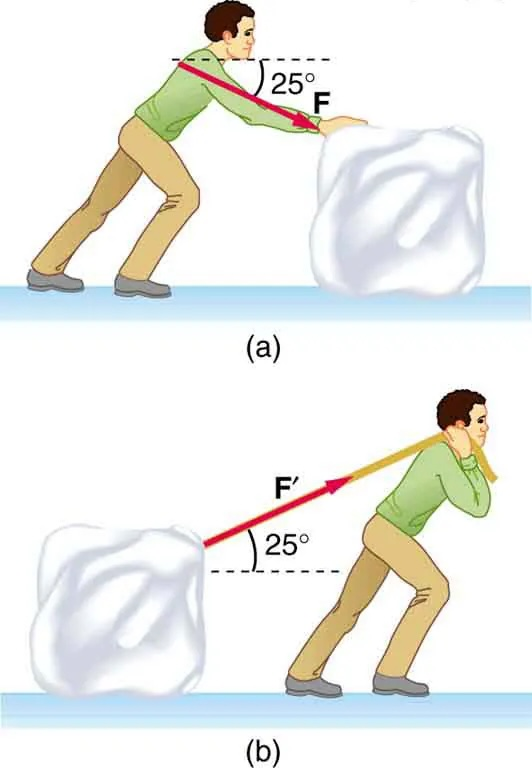
\includegraphics[width=1.8in]{OpenStaxImages/5-21.jpg}
      \caption{Which method of sliding a block of ice requires less force—(a) pushing or (b) pulling at the same angle above the horizontal?}
    \end{figure}

  % \myquestion
  %   (OpenStax Ex 5.8) Show that the acceleration of any object down a frictionless incline that makes an angle $\theta$ with the horizontal is $a=g\sin\theta$. (Note that this acceleration is independent of mass.)   
  
  % \myquestion
  %   (OpenStax Ex 5.9) Show that the acceleration of any object down an incline where friction behaves simply (that is, where $f_k=\mu_k N$) is $a=g\left( \sin\theta - \mu_k \cos\theta \right)$.  Note that the acceleration is independent of mass and reduces to the expression found in the previous problem when friction becomes negligibly small ($\mu_k=0$).

  % \myquestion
  %   (OpenStax Ex 5.10) Calculate the deceleration of a snow boarder going up a $5.0^\circ$, slope assuming the coefficient of friction for waxed wood on wet snow. The result of the previous problem may be useful, but be careful to consider the fact that the snow boarder is going uphill. \answer{\SI{1.83}{m/s^2}}

  \myquestion
    (OpenStax Ex 5.11) (a) Calculate the acceleration of a skier heading down a $10^\circ$ slope, assuming the coefficient of friction for waxed wood on wet snow. (b) Find the angle of the slope down which this skier could coast at a constant velocity. \answer{$5.71^\circ$}
  
  \begin{enumerate}
    \item[CQ-C)] (Original Question) Look above at Figure 5-21.  Which method of moving the block would be easier: pulling from in front or pushing from the back? Explain.
    \item[CQ-D)] (Original Question) One block sits at rest on a level surface while a second identical block sits at rest on an incline.  In which case is the normal force larger?  Why?
  \end{enumerate}

  \myquestion
    \textbf{Bonus!} (OpenStax Ex 5.12) If an object is to rest on an incline without slipping, then friction must equal the component of the weight of the object parallel to the incline. This requires greater and greater friction for steeper slopes. Show that the maximum angle of an incline above the horizontal for which an object will not slide down is $\theta=\tan^{-1}\mu_s$. You may use the result of the previous problem. Assume that $a=0$ and that static friction has reached its maximum value.

  \myquestion
    \textbf{Bonus!} (OpenStax Ex 4.42) A 76.0-kg person is being pulled away from a burning building as shown in Figure 4.40. Calculate the tension in the two ropes if the person is momentarily motionless. Include a free-body diagram in your solution.

    \begin{figure}[h]
      \centering
      \renewcommand{\thefigure}{4.40}
      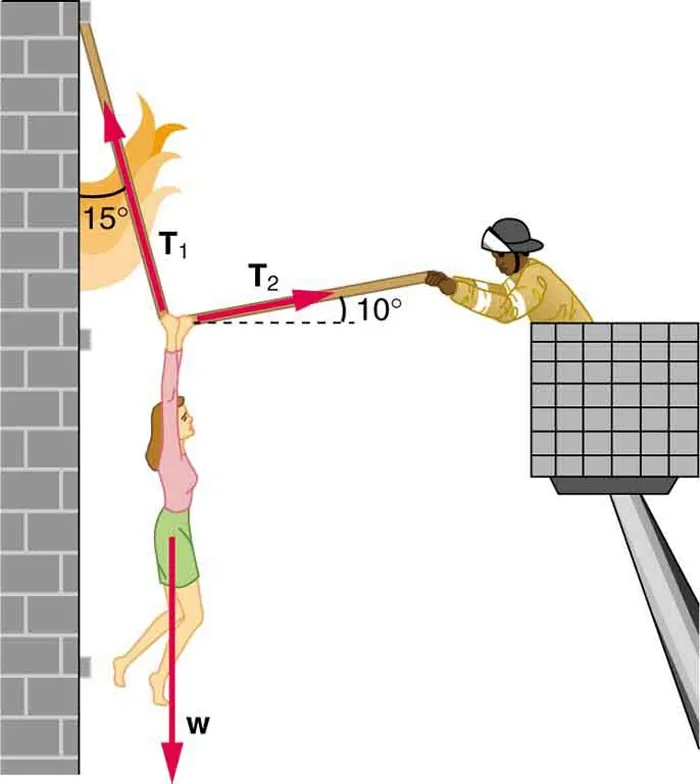
\includegraphics[width=1.9in]{OpenStaxImages/4-40.jpg}
      \caption{The force $T_1$ needed to hold steady the person being rescued from the fire is less than her weight and less than the force $T_2$ in the other rope, since the more vertical rope supports a greater part of her weight (a vertical force).}
    \end{figure}


\uplevel{
  \section*{Additional Practice Problems}

  \textit{These problems are not required and are not bonus. Worked out solutions are available on Schoology.}

}

    \myquestion
      (Problem 4-19 from Giancolli \textit{Physics: Principles with Applications}, 7th ed.) The cable supporting a 2125-kg elevator has a maximum strength of 21,750~N.  What maximum upward acceleration can it give without breaking? \answer{\SI{0.44}{m/s^2}}

    \myquestion
      (Problem 4-37 from Giancolli) A force of 35.0~N is required to start a 6.0-kg box moving across a horizontal concrete floor.  (a) What is the coefficient of static friction between the box and the floor?  (b) If the 35.0-N force continues, the box accelerates at \SI{0.60}{m/s^2}. What is the coefficient of kinetic friction? \answer{(a) $\mu_s=0.60$ (b) $\mu_k=0.53$}

    \myquestion
      (Problem 4-25 from Giancolli) One 3.2-kg paint bucket is hanging by a massless cord from another 3.2-kg paint bucket, also hanging by a massless cord, as shown in Figure~4-49.  (a) If the massless buckets are at rest, what is the tension on each cord?  (b) If the two buckets are pulled upward with an acceleration of \SI{1.25}{m/s^2} by the upper cord, calculate the tension on each cord. \answer{(a) 31.36 N and 62.72 N; (b) 35.36 N and 70.72 N}

      \begin{figure}[h]
        \centering
        \renewcommand{\thefigure}{4-49}
        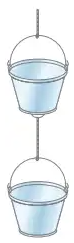
\includegraphics[height=1.6in]{OpenStaxImages/Giancolli4-49.png}
        \caption{From Giancolli}
      \end{figure}

    \myquestion
        (Problem 4-49 from Giancolli, modified) Two crates of mass 65~kg and 125~kg are in contact and at rest on a horizontal surface (Figure~4-57).  A 650-N force is exerted on 65-kg crate.  Calculate (a) the acceleration of the system and (b) the force that each crate exerts on the other.  (c) Repeat with the crates reversed. \answer{(a) \SI{3.42}{m/s^2} (b) \SI{427.5}{N} (c) \SI{3.42}{m/s^2} and \SI{22.3}{N} }

        \begin{figure}[h]
          \centering
          \renewcommand{\thefigure}{4-57}
          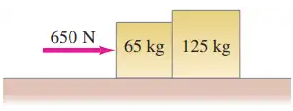
\includegraphics[width=2in]{OpenStaxImages/Giancolli4-57.png}
          \caption{From Giancolli}
        \end{figure}
    


\end{questions}


\end{document}